\documentclass[11pt,a4paper]{article}
\usepackage[T1]{fontenc}
\usepackage{ae}
\usepackage[utf8]{inputenc}
\usepackage{amsmath,amssymb}
\usepackage[margin=2.6cm]{geometry}
\IfFileExists{infwarerr.sty}{
  \usepackage[unicode,hidelinks]{hyperref}
}{
  \usepackage{url}
  \newcommand{\href}[2]{\leavevmode\pdfstartlink attr{/Border [0 0 0]} user{/Subtype /Link /A << /S /URI /URI (##1) >>}##2\pdfendlink}
}
\usepackage{graphicx}
\graphicspath{{figure/}{docs/apertura-ricerca/figure/}}
\IfFileExists{italian.ldf}{\usepackage[italian]{babel}}{\usepackage{babel}\babelprovide[import,main]{italian}}
\renewcommand{\contentsname}{Indice}
\renewcommand{\refname}{Riferimenti iniziali}
\setlength{\emergencystretch}{3em}
\postdisplaypenalty=500
\newcommand{\Sol}{\operatorname{Sol}}
\newcommand{\Pareto}{\operatorname{Pareto}}
\newcommand{\Wild}{\bot}
\title{Ricerca sulla complessità dei problemi di tiling\\[0.4em]
\large Definizione dello spazio dei problemi, transizioni e intenti di ricerca}
\author{magn.manuel05}
\date{Ottobre 2026}
\begin{document}
\maketitle

\section{Introduzione}

Si vuole definire un ambiente di comparazione e studio del comportamento dei tiling al variare dei vincoli di costruzione del problema.

Si auspica come successo della ricerca la definizione di uno spazio dei problemi che sia sufficientemente capiente per contenere una classe quanto più ampia possibile di istanze finite di tiling, con vari sottoinsiemi più stringenti per studiare particolari proprietà o relazioni tra i vincoli. L'interesse è anche quello di comprendere quali famiglie di problemi computazionali possano essere rappresentate in questo spazio, attraverso codifiche da rendere esplicite e da studiare separatamente.

Un altro criterio di riuscita di questa ricerca è quello di definire quantità in funzione di un problema che restituiscano valori numerici rappresentativi della sua complessità o espressività. Con queste si vorrebbero innanzitutto studiare famiglie di problemi di cui conosciamo alcune proprietà e poi costruire una metodologia di comparazione tra variazioni nei vincoli.

Il presente testo propone le definizioni di partenza e le domande che si intendono indagare. Viene accompagnato da Wang Studio, un editor sviluppato per costruire istanze e condurre i primi esperimenti. 

\section{Definizione dello spazio dei problemi}

Il motivo di questa ridefinizione di un problema molto conosciuto è che, a partire dal problema del domino di Wang sul piano infinito, si sono sviluppate varianti con regioni, tessere e condizioni di bordo differenti. Il problema sul piano infinito è indecidibile in generale~\cite{berger}. Essendo lo scopo della ricerca quello di esplorare i vincoli di diverse versioni, ritengo necessario definire uno spazio comune nel quale confrontarle.

In questa prima formulazione si considerano regioni finite, tileset finiti e posizionamenti discreti. Il problema decisionale è pertanto decidibile tramite enumerazione delle configurazioni.

\subsection{Vincoli generali}

Un problema dello spazio deve presentare un insieme finito di colori, un insieme finito di tessere e una regione finita non vuota. Le tessere atomiche sono poligoni regolari che formano una tassellazione del piano lato a lato di un solo tipo: triangoli equilateri, quadrati oppure esagoni regolari. Indichiamo con
\[
s\in\{3,4,6\}
\]
il numero di lati di una tessera atomica.

Le tessere possono essere traslate e utilizzate un numero arbitrario di volte, ma non possono essere ruotate o riflesse durante il posizionamento. Eventuali orientamenti differenti devono essere specificati nella definizione dei tipi ammessi. Le tessere generalizzate sono composizioni finite di celle di una sola geometria atomica; per esse si introdurrà un ulteriore vincolo di unicità della soluzione interna.

\subsection{Ambiente geometrico}

Fissiamo una tassellazione regolare del piano di geometria $s$ e indichiamo con $Q_v\subseteq\mathbb R^2$ la cella chiusa corrispondente alla posizione $v$. Il suo grafo di adiacenza è
\[
G_s=(V_s,E_s,o_s),
\qquad E_s\subseteq(V_s\times[s])^2,
\qquad [s]=\{1,\ldots,s\}.
\]
La coppia $((u,i),(v,j))\in E_s$ indica che il lato $i$ di $Q_u$ coincide con il lato $j$ di $Q_v$. La relazione è simmetrica e ciascun lato ha al più un adiacente. La funzione $o_s$ specifica il tipo di orientamento della cella.

Fissiamo verso e lato iniziale della numerazione dei lati; l'editor utilizza per i quadrati l'ordine $(N,E,S,W)$. Per i triangoli sono presenti due tipi di orientamento e una tessera può occupare soltanto celle del proprio tipo. L'editor condivide le tuple fra i due orientamenti locali: nel modello a tipi distinti questa convenzione equivale a includere, per ogni tupla, una tessera di ciascun tipo.

La regione geometrica associata a $R\subseteq V_s$ è
\[
A_R=\bigcup_{v\in R}Q_v.
\]
Nel confronto fra forme identifichiamo le traslazioni, mantenendo distinte rotazioni e riflessioni. La regione come insieme di celle $R$ e la sua realizzazione continua $A_R$ sono oggetti distinti: la seconda permette di confrontare geometrie atomiche differenti nello stesso piano. La normalizzazione e l'allineamento usati nella transizione sono precisati nella sezione~\ref{sec:campo-continuo}.

\subsection{Colori e condizioni di bordo}

Sia $\Sigma$ un insieme numerabile di simboli e sia $C\subseteq\Sigma$ un insieme finito non vuoto di colori. Il vincolo cromatico è l'uguaglianza fra simboli. Una rinomina biettiva applicata coerentemente a tessere e bordo conserva le soluzioni.

Una regione è un sottoinsieme finito non vuoto $R\subseteq V_s$, connesso rispetto alle adiacenze. Il suo bordo è
\[
B_R=\left\{(v,i)\in R\times[s]\;\middle|\;
\nexists u\in R,\ j\in[s]:((v,i),(u,j))\in E_s\right\}.
\]
Il numero $|B_R|$ conta i lati atomici esposti, compresi quelli rivolti verso eventuali buchi.

Per comprendere anche i bordi parzialmente vincolati dell'editor, definiamo
\[
\beta:B_R\longrightarrow C\cup\{\Wild\},
\qquad \Wild\notin C.
\]
Il simbolo $\Wild$ indica assenza di vincolo, rappresentata nell'editor mediante un tratteggio.

\begin{figure}[htbp]
\centering
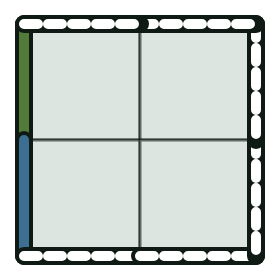
\includegraphics[width=3.5cm]{bordo-parziale.png}
\caption{Regione quadrata di quattro celle con due lati vincolati, verde e blu, e sei lati senza vincolo. I tratti tratteggiati delimitano la regione senza imporre un colore. Nelle figure il riempimento grigio evidenzia le celle della regione.}
\label{fig:bordo}
\end{figure}


Lo spazio generale può comprendere regioni con buchi. La transizione geometrica attualmente studiata viene però definita sul sottoinsieme delle regioni con un unico contorno semplice: buchi, contatti singolari del contorno e componenti disconnesse non rientrano nel suo dominio.

\subsection{Problema atomico e insieme delle soluzioni}

Un problema atomico è una tupla
\[
P=(G_s,C,T,R,\beta).
\]
Quando vi è un solo tipo di orientamento, lo spazio dei tileset atomici è l'insieme delle parti di $C^s$:
\[
\mathcal T_{s,C}:=\operatorname{Pow}(C^s)=2^{C^s}.
\]
Un tileset e le sue tessere soddisfano quindi
\[
\boxed{T\in\mathcal T_{s,C},\qquad t\in T\implies t\in C^s.}
\]
Poiché $C$ è finito, ogni tileset così definito è finito. Nel modello con tipi distinti, una tessera è una coppia $(o,t)$ con $t\in C^s$, e il posizionamento deve rispettare anche $o_s$; lo spazio dei tileset è allora l'insieme delle parti dell'insieme delle tessere tipate ammesse.

Un'assegnazione $\tau:R\to T$ è una soluzione se è compatibile con gli orientamenti e soddisfa
\[
\tau(u)_i=\tau(v)_j
\quad\text{per ogni }((u,i),(v,j))\in E_s\text{ con }u,v\in R,
\]
nonché
\[
\tau(v)_i=\beta(v,i)
\quad\text{per ogni }(v,i)\in B_R\text{ con }\beta(v,i)\neq\Wild.
\]
Qui $\tau(v)_i$ indica il colore del lato $i$, anche quando il tipo è incluso nella tessera. Denotiamo con $\Sol(P)$ l'insieme delle soluzioni. Il problema decisionale chiede se $\Sol(P)\neq\varnothing$; il problema di conteggio chiede di determinare $|\Sol(P)|$.

Il numero di assegnazioni da considerare è al più $|T|^{|R|}$. La figura~\ref{fig:soluzione-atomica} mostra un esempio di compatibilità locale e di bordo.

\begin{figure}[htbp]
\centering
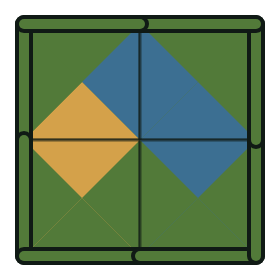
\includegraphics[width=3.6cm]{soluzione-atomica.png}
\caption{Una soluzione su quattro celle. Ogni settore triangolare indica il colore di un lato della tessera quadrata: i settori che si toccano hanno lo stesso colore e tutti i lati esterni rispettano il bordo verde. Le diagonali sono una convenzione grafica, non suddivisioni in celle triangolari.}
\label{fig:soluzione-atomica}
\end{figure}


\subsection{Tessere generalizzate}

Una tessera generalizzata è specificata da un problema atomico finito
\[
g=(G_s,C,T_g,R_g,\beta_g)
\]
il cui bordo è interamente colorato e per il quale richiediamo
\[
\boxed{|\Sol(g)|=1.}
\]
L'unicità della soluzione interna è un vincolo scelto per questa ricerca.

La forma e il bordo descrivono il comportamento esterno della tessera; $T_g$ e la soluzione unica ne specificano la realizzazione interna (figura~\ref{fig:generalizzata}).

\begin{figure}[htbp]
\centering
\begin{minipage}{0.44\textwidth}
\centering
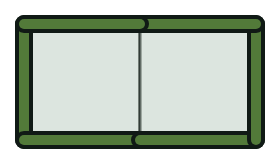
\includegraphics[width=4.2cm]{generalizzata-bordo.png}\\[0.4em]
(a) Forma e bordo assegnati
\end{minipage}\hfill
\begin{minipage}{0.44\textwidth}
\centering
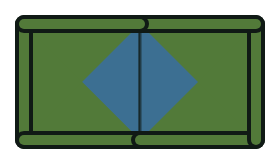
\includegraphics[width=4.2cm]{generalizzata-interno.png}\\[0.4em]
(b) Unica soluzione interna
\end{minipage}
\caption{Esempio atomico che soddisfa la definizione di tessera generalizzata. Con $v$ verde e $b$ blu, si usa $T_g=\{(v,b,v,v),(v,v,v,b)\}$ nell'ordine $(N,E,S,W)$. Il bordo interamente verde forza la prima tessera a sinistra e la seconda a destra, con contatto blu. Delle quattro assegnazioni possibili, esattamente una è valida. Il grigio in (a) indica soltanto la regione. L'editor rappresenta qui la realizzazione atomica, non un pezzo indivisibile.}
\label{fig:generalizzata}
\end{figure}


Indichiamo con $\mathcal G_s$ lo spazio delle generalizzate ammissibili. Un tileset di generalizzate è un sottoinsieme finito di $\mathcal G_s$; una soluzione con tali pezzi deve coprire la regione senza sovrapposizioni, usando soltanto traslazioni compatibili con la griglia e rispettando i colori lungo i contatti. Si possono studiare anche tileset misti di pezzi atomici e generalizzati.

L'equivalenza fra un tileset di generalizzate e l'unione $\bigcup_g T_g$ richiede vincoli che ne preservino la decomposizione in pezzi: l'unicità interna non esclude assemblaggi atomici che attraversino i loro confini. Si vorrebbero studiare le condizioni che garantiscono questa equivalenza.

Ritengo inoltre rilevante il sottoinsieme delle tessere generalizzate convesse. Posto
\[
A_g=A_{R_g}=\bigcup_{v\in R_g}Q_v,
\]
definiamo
\[
\mathcal G_s^{\mathrm{conv}}=
\left\{g\in\mathcal G_s:\
(1-\lambda)x+\lambda y\in A_g\quad
\forall x,y\in A_g,\ \forall\lambda\in[0,1]\right\}.
\]
Non è ancora stabilito se questo sottoinsieme verrà trattato, ma potrebbe offrire un ambiente più stringente qualora lo studio del caso generale risultasse troppo variabile.

\begin{figure}[htbp]
\centering
\begin{minipage}[b]{0.42\textwidth}
\centering
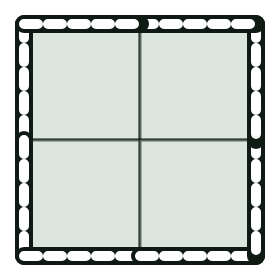
\includegraphics[width=3.5cm]{regione-convessa.png}\\[0.4em]
(a) Regione convessa
\end{minipage}\hfill
\begin{minipage}[b]{0.42\textwidth}
\centering
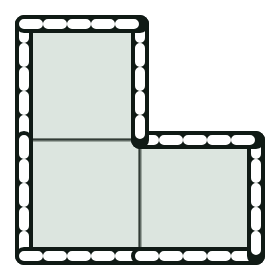
\includegraphics[width=3.5cm]{regione-concava.png}\\[0.4em]
(b) Regione non convessa
\end{minipage}
\caption{Due regioni costruite nell'editor. Nel rettangolo ogni segmento fra punti della regione rimane al suo interno; nella forma a L alcuni segmenti attraversano la cella mancante. Il confronto riguarda la forma $A_R$; per ottenere tessere generalizzate occorre scegliere bordo e tileset e verificarne la soluzione unica.}
\label{fig:convessita}
\end{figure}


\section{Variazione dei vincoli}

Definito un problema di tiling, procediamo a chiarire cosa significhi muoversi nello spazio di ciascun vincolo. L'obiettivo è descrivere operazioni ammissibili, distinguendo le proprietà che vengono mantenute da quelle che possono cambiare.

I vincoli non sono indipendenti: l'insieme dei colori determina i valori ammessi nelle tessere e sul bordo; la regione determina il dominio della colorazione di bordo; la geometria determina il numero e le adiacenze dei lati. Una variazione può quindi richiedere l'adattamento di altri componenti. 

\subsection{Colorazioni}

Possiamo aggiungere o rimuovere simboli da $C$. Considerando soltanto la cardinalità, il minimo spostamento non nullo è $1$. Questo parametro non descrive però tutto l'effetto della variazione: aggiungere un colore non utilizzato non cambia le soluzioni, mentre rimuovere un colore presente nelle tessere o nel bordo richiede di modificarne gli usi.

Si vorrebbero quindi distinguere variazioni della palette, sostituzioni nei vincoli e fusioni di colori prima diversi. Quest'ultima operazione può modificare quali lati risultano compatibili. La semplice rinomina biettiva, invece, dovrebbe essere riconosciuta come equivalenza di rappresentazione.

\subsection{Tessere}

A geometria e palette fissate, muoversi fra tileset atomici significa passare da un elemento $T$ a un altro elemento $T'$ dello spazio $\mathcal T_{s,C}=2^{C^s}$, aggiungendo o eliminando tuple ammesse. Possiamo misurare lo spostamento attraverso
\[
d_T(T,T')=|T\triangle T'|.
\]
Il minimo spostamento non nullo è $1$, purché il risultato appartenga al sottoinsieme che si sta studiando. Per le generalizzate, l'aggiunta richiede anche la verifica del vincolo di unicità.

Un tileset atomico può essere rappresentato mediante un vettore indicatore
\[
\chi_T\in\{0,1\}^{|C|^s},
\]
nel caso a un solo tipo, ottenendo uno spazio combinatorio per confrontare tileset.

Sarebbe interessante studiare la ridondanza di una tessera rispetto a una famiglia di istanze, considerando sia la tesserabilità sia il numero delle soluzioni.

\subsection{Regione}

A geometria fissata, un'operazione elementare consiste nell'aggiungere o rimuovere una cella, mantenendo i requisiti di connessione e, quando richiesti, quelli sul contorno. L'operazione comprende anche una scelta delle condizioni sui nuovi lati esposti.

Misurando l'area in numero di celle, il minimo incremento positivo è $1$. Se una cella aggiunta condivide $k$ lati con la regione esistente, la variazione del numero di lati esposti è
\[
\boxed{\Delta B=s-2k.}
\]
La stessa operazione può quindi aumentare, diminuire o lasciare invariato il bordo (figura~\ref{fig:variazione-perimetro}). La quantità $\bigl||B_R|-|B_{R'}|\bigr|$ misura una differenza di perimetro combinatorio, ma non è una distanza fra forme: regioni differenti possono avere lo stesso valore.

Ritengo interessante studiare come area, bordo e condizioni cromatiche possano essere controllati separatamente e come le loro variazioni influenzino tesserabilità e numero delle soluzioni.

\begin{figure}[htbp]
\centering
\begin{tabular}{c@{\quad}c@{\quad}c@{\quad}c}
 & Prima & Dopo & Variazione \\[0.6em]
$k=1$ & 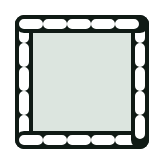
\includegraphics[height=1.25cm]{perimetro-k1-prima.png} & 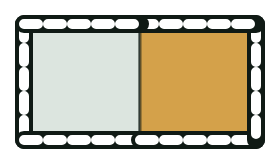
\includegraphics[height=1.25cm]{perimetro-k1-dopo.png} & $B:4\to6$ \\[0.6em]
$k=2$ & 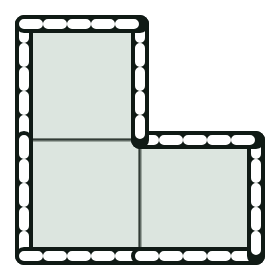
\includegraphics[height=2.2cm]{perimetro-k2-prima.png} & 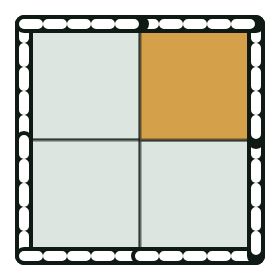
\includegraphics[height=2.2cm]{perimetro-k2-dopo.png} & $B:8\to8$ \\[0.6em]
$k=3$ & 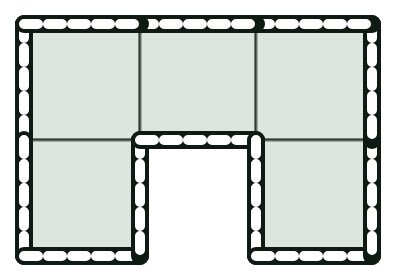
\includegraphics[height=2.2cm]{perimetro-k3-prima.png} & 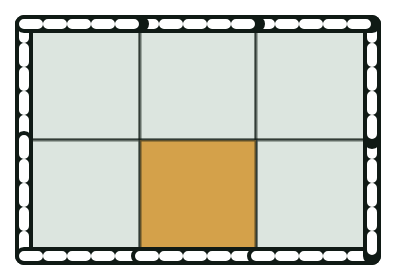
\includegraphics[height=2.2cm]{perimetro-k3-dopo.png} & $B:12\to10$
\end{tabular}
\caption{Aggiungere una cella aumenta sempre $|R|$ di uno, ma può aumentare, lasciare invariato o diminuire il bordo. La cella ocra condivide rispettivamente uno, due o tre lati con la regione grigia: $\Delta B=4-2k$ vale $+2$, $0$ e $-2$. I riempimenti distinguono le celle a scopo illustrativo e non indicano vincoli cromatici; tutti i lati esterni sono jolly.}
\label{fig:variazione-perimetro}
\end{figure}

\section{Variazione della geometria e funzione di transizione}
\label{sec:transizione}

Cambiare geometria significa passare da un problema definito su $G_s$ a uno definito su $G_{s'}$, trasformando regione, adiacenze, bordo e tileset.

Definiamo lo spostamento mediante una relazione di ammissibilità, fissando gli invarianti e i criteri con cui selezionare le realizzazioni.

\subsection{Dati conservati e dominio della transizione}

La prima transizione studiata conserva le interfacce di bordo, lascia libere le adiacenze interne e ricostruisce il tileset di destinazione.

Per seguire il bordo anche attraverso più transizioni introduciamo una lista ciclica di interfacce distinte
\[
\Lambda=(\lambda_0,\ldots,\lambda_{m-1}),
\qquad c:\Lambda\to C\cup\{\Wild\},
\]
e una corrispondenza $q:B_R\to\Lambda$ che ne descrive la realizzazione corrente, con $\beta=c\circ q$. Inizialmente ogni lato è un'interfaccia distinta e $q$ è biiettiva. Interfacce con lo stesso colore non vengono fuse.

La transizione opera dunque sui dati di bordo arricchiti
\[
X=(G_s,R,\Lambda,c,q).
\]
Le interfacce conservano identità, ordine ciclico e colore. Nella convenzione scelta, ciascuna interfaccia colorata occupa esattamente un lato atomico; quelle senza vincolo possono occupare più lati consecutivi. Il numero di lati vincolati di ciascun colore rimane quindi invariato.

\subsection{Normalizzazione dell'area e rapporto di contatto}

Assumiamo che le celle atomiche abbiano circumraggio unitario. L'area di una cella di geometria $s$ è
\[
a_s=\frac{s}{2}\sin\left(\frac{2\pi}{s}\right),
\qquad A(R)=|R|a_s.
\]
La normalizzazione è una scelta del modello, indipendente dalla scala del disegno nell'editor. Per una destinazione di geometria $s'$, il numero ideale di celle è
\[
N^*=|R|\frac{a_s}{a_{s'}}.
\]

Indichiamo con $B(R)=|B_R|$ il numero di lati esterni e con $I(R)$ il numero di coppie di celle adiacenti, contando ciascun contatto una sola volta. Vale
\[
s|R|=2I(R)+B(R).
\]
Definiamo
\[
\rho(R)=\begin{cases}B(R)/I(R),&I(R)>0,\\+\infty,&I(R)=0.\end{cases}
\]
Si vuole conservare approssimativamente il rapporto della sorgente.

Per due regioni $R,S$, definiamo
\[
\delta_A(R,S)=\frac{|A(S)-A(R)|}{A(R)}
\]
e, quando entrambi i rapporti sono finiti,
\[
\delta_\rho(R,S)=
\frac{|\rho(S)-\rho(R)|}{\max\{\rho(S),\rho(R)\}}.
\]
Per convenzione, $\delta_\rho=0$ quando entrambi sono infiniti e $\delta_\rho=1$ quando esattamente uno è infinito.

Fissate le tolleranze $\varepsilon\geq0$ e $0\leq\tau\leq1$, imponiamo
\[
\delta_A(R,S)\leq\varepsilon,
\qquad \delta_\rho(R,S)\leq\tau.
\]
L'area determina l'intervallo di dimensioni
\[
N_{\min}=\max\{1,\lceil(1-\varepsilon)N^*\rceil\},
\qquad N_{\max}=\lfloor(1+\varepsilon)N^*\rfloor.
\]
Un intervallo vuoto esclude ogni realizzazione entro la tolleranza scelta.

\subsection{Riferimento continuo e allineamento delle regioni}
\label{sec:campo-continuo}

Area e rapporto di contatto non descrivono da soli la disposizione della regione nel piano. Una regione a C e una regione allungata possono avere la stessa area e lo stesso rapporto $B/I$, pur occupando porzioni del piano molto diverse. Si vuole introdurre una quantità che renda osservabile questa differenza, lasciando a ciascuna geometria la possibilità di esprimersi senza riprodurre esattamente il contorno sorgente.

Usiamo come riferimento l'unione continua $A_R=\bigcup_{v\in R}Q_v$, già introdotta nella definizione dell'ambiente geometrico. Tutti i poligoni sono ora espressi nella normalizzazione del circumraggio unitario. Se una rappresentazione grafica usa circumraggio $r_s^{\mathrm{graf}}$, le sue coordinate devono essere moltiplicate per
\[
\frac{1}{r_s^{\mathrm{graf}}}.
\]
In Wang Studio i circumraggi grafici sono rispettivamente $1/\sqrt{3}$, $1/\sqrt{2}$ e $1$ per triangoli, quadrati ed esagoni. Il confronto avviene quindi in uno spazio euclideo comune, coerente con le aree $A(R)$ e $A(S)$, e non nelle coordinate grezze del canvas.

Posto $\mu_2$ per l'area euclidea, il centroide geometrico e la regione allineata sono
\[
\bar x_R=\frac{1}{A(R)}\int_{A_R}x\,\mathrm dx,
\qquad \Omega_R=A_R-\bar x_R,
\qquad \mu_2(\Omega_R)=A(R).
\]
Definiamo nello stesso modo $\Omega_S$. Poiché le celle di ciascuna regione hanno uguale area, il centroide è anche la media dei loro centroidi. Le due regioni vengono confrontate con i centroidi nell'origine, indipendentemente dalla posizione assoluta del disegno. Non applichiamo riscalamenti per uguagliare le aree, rotazioni ottimizzate o riflessioni. Questa convenzione conserva l'orientamento geometrico delle interfacce.

La distanza firmata dalla sorgente è
\[
d_R(x)=
\begin{cases}
-\operatorname{dist}(x,\partial\Omega_R),&x\in\Omega_R,\\
\phantom{-}\operatorname{dist}(x,\partial\Omega_R),&x\notin\Omega_R.
\end{cases}
\]
Il bordo $\partial\Omega_R$ è quello dell'unione dei poligoni: i lati interni fra celle non vi contribuiscono. La regione continua mantiene quindi anche rientranze e parti non convesse; non viene sostituita dal rettangolo che la contiene.

Fissata una percentuale $p_\sigma\geq0$, poniamo
\[
\boxed{\sigma=\frac{p_\sigma}{100}\sqrt{A(R)}.}
\]
Per $\sigma>0$ introduciamo il campo continuo
\[
\boxed{\phi_\sigma(x)=
\operatorname{clip}\!\left(\frac12-\frac{d_R(x)}{2\sigma},0,1\right),}
\qquad
\operatorname{clip}(z,0,1)=\min\{1,\max\{0,z\}\}.
\]
Il valore è $1$ almeno a distanza $\sigma$ all'interno della sorgente e $0$ almeno a distanza $\sigma$ all'esterno. La fascia di transizione si estende di $\sigma$ su ciascun lato del bordo. Per $p_\sigma=0$ adottiamo il limite $\phi_0=\mathbf1_{\Omega_R}$ quasi ovunque: la scelta del valore sul bordo non modifica gli integrali di area. Il riferimento rimane una regione continua, anche se questo campo limite è discontinuo sul contorno.

\subsection{Errore geometrico, preferenza e vincolo di forma}
\label{sec:errore-forma}

La differenza integrata fra l'indicatrice della destinazione e il campo morbido non sarebbe nulla nemmeno per la sorgente stessa. Definiamo invece l'errore sulla differenza simmetrica delle regioni allineate:
\[
\boxed{
E_\sigma(R,S)=\frac{1}{A(R)}
\int_{\Omega_R\triangle\Omega_S}
\min\!\left(1,\frac{|d_R(x)|}{\sigma}\right)\,\mathrm dx,
\qquad \sigma>0.}
\]
Nel limite netto poniamo
\[
\boxed{E_0(R,S)=
\frac{\mu_2(\Omega_R\triangle\Omega_S)}{A(R)}.}
\]
Le porzioni aggiunte all'esterno e quelle mancanti all'interno contribuiscono entrambe. Vicino al bordo il costo cresce gradualmente; oltre la fascia raggiunge il valore unitario per unità di area. Se $\Omega_R=\Omega_S$, l'errore è zero per ogni larghezza della fascia, anche quando i disegni originali differiscono per una traslazione.

La normalizzazione dipende dall'area della sorgente e non dal numero di tessere di destinazione. In particolare
\[
0\leq E_\sigma(R,S)\leq E_0(R,S)
\leq 1+\frac{A(S)}{A(R)}.
\]
L'errore può quindi superare il $100\%$. A regioni fissate è non crescente all'aumentare di $\sigma$; per $\sigma\to0^+$ tende a $E_0$, poiché il bordo poligonale ha area nulla. Non lo assumiamo come una metrica: il riferimento, la normalizzazione e la larghezza della fascia dipendono dalla sorgente, per cui in generale il confronto non è simmetrico.

Introduciamo una seconda percentuale, indipendente da $p_\sigma$:
\[
\boxed{\tau_E=\frac{p_E}{100},\qquad p_E\geq0.}
\]
$p_\sigma$ controlla la morbidezza spaziale del riferimento; $p_E$ controlla la quantità complessiva di errore ammessa quando si richiede il vincolo $E_\sigma(R,S)\leq\tau_E$.

Per separare i due usi della misura, indichiamo con $\alpha\in\{0,1\}$ l'attivazione della preferenza geometrica e con $\kappa\in\{0,1\}$ l'attivazione del vincolo rigido. La preferenza aggiunge l'errore di forma agli obiettivi di confronto, senza escludere automaticamente i candidati lontani; il vincolo restringe invece l'ammissibilità. Le due scelte possono essere attivate separatamente. Nel seguito raccogliamo i parametri matematici in
\[
\vartheta=(\varepsilon,\tau,p_\sigma,p_E,\alpha,\kappa).
\]
L'errore geometrico è un osservabile distinto da area e rapporto di contatto. Non introduciamo ulteriori vincoli di convessità, scheletro, diametro o assi principali per la transizione. L'eventuale studio delle generalizzate convesse rimane un sottoinsieme separato dello spazio dei problemi.

\subsection{Spazio delle realizzazioni ammissibili}

Una realizzazione di bordo è una coppia $(S,p)$, dove $S$ è una regione della geometria $s'$ e
\[
p:B_S\longrightarrow\Lambda
\]
associa i lati di destinazione alle interfacce sorgenti. Richiediamo che $p$ sia suriettiva e conservi l'ordine ciclico, e che la fibra di ogni interfaccia sia un tratto consecutivo non vuoto del contorno. Inoltre
\[
|p^{-1}(\lambda_i)|=1\quad\text{se }c(\lambda_i)\neq\Wild,
\qquad \beta_S=c\circ p.
\]
Le rotazioni del punto iniziale della lista sono consentite; l'inversione dell'ordine non lo è. Definiamo
\[
\mathcal R_{s'}^{\varepsilon,\tau}(X)=
\left\{(S,p)\;\middle|\;
\begin{array}{l}
S\text{ è finita, connessa, con un unico contorno semplice},\\
p\text{ soddisfa le condizioni sulle interfacce},\\
\delta_A(R,S)\leq\varepsilon,\quad\delta_\rho(R,S)\leq\tau
\end{array}\right\}.
\]
A meno di traslazioni, questo insieme è finito: vi è un limite superiore al numero di celle, ogni cella ha un numero finito di vicini e, per ogni forma, vi è un numero finito di corrispondenze di bordo.

La nuova famiglia ammissibile è
\[
\boxed{\mathcal R_{s'}^{\vartheta}(X)=
\left\{(S,p)\in\mathcal R_{s'}^{\varepsilon,\tau}(X):
\kappa=0\ \text{oppure}\ E_\sigma(R,S)\leq\tau_E\right\}.}
\]
Per $\kappa=0$ si recupera lo spazio precedente; $\alpha$ non ne modifica il dominio. La regione continua sorgente serve da riferimento quantitativo, senza richiedere che $\Omega_S$ ne riproduca esattamente il contorno. La completezza della ricerca viene studiata rispetto a questo spazio di regioni e corrispondenze di bordo, a sorgente e parametri fissati.

Se $m=|\Lambda|$, $b=B(S)$ e $w$ è il numero di interfacce senza vincolo, la capacità del bordo richiede
\[
b\geq m,\qquad w=0\Longrightarrow b=m.
\]
Per un contorno semplice fissato queste condizioni permettono una distribuzione delle interfacce: ogni interfaccia riceve un lato e gli eventuali lati rimanenti vengono assegnati a quelle senza vincolo.

\subsection{Proprietà della transizione}

La mappa di bordo $p$ è suriettiva ed è biiettiva esattamente quando $b=m$.

La corrispondenza $X\mapsto\mathcal R_{s'}^{\vartheta}(X)$ è a valori insiemistici. Una regola di selezione ne determina una funzione parziale quando l'insieme è non vuoto. La preferenza geometrica modifica il confronto fra le realizzazioni, mentre soltanto $\kappa=1$ aggiunge una condizione di ammissibilità sulla forma.

Spostarsi nella geometria significa scegliere un elemento di $\mathcal R_{s'}^{\vartheta}(X)$. Le quantità $\delta_A$, $\delta_\rho$ ed $E_\sigma$ descrivono aspetti distinti dello spostamento, senza costituire una distanza completa fra problemi: non misurano, per esempio, la variazione del tileset o delle soluzioni.

A sorgente e geometria di destinazione fissate, allargare le tolleranze può soltanto ampliare lo spazio ammissibile. Più precisamente, a $p_\sigma$, $\alpha$ e $\kappa$ fissati,
\[
\varepsilon_1\leq\varepsilon_2,\quad \tau_1\leq\tau_2,
\quad p_{E,1}\leq p_{E,2}
\quad\Longrightarrow\quad
\mathcal R_{s'}^{\vartheta_1}(X)
\subseteq\mathcal R_{s'}^{\vartheta_2}(X).
\]
Quando $\kappa=0$, $p_E$ non modifica l'insieme. Aumentare $p_\sigma$ indebolisce il costo delle deformazioni e, a soglia di forma fissata, non restringe l'ammissibilità; non equivale però a cambiare $p_E$, perché modifica anche i valori dell'obiettivo geometrico.

Quando la griglia di destinazione coincide con quella sorgente, inclusa la convenzione di orientamento, la realizzazione corrente $(R,q)$ appartiene allo spazio ammissibile con tutti e tre gli errori nulli. Non assumiamo reversibilità né invertibilità. Una successione di transizioni può accumulare scostamento, perché ciascun passo usa la regione corrente come nuovo riferimento. Un ritorno alla geometria iniziale non implica il recupero della forma o del tileset iniziali.

La conservazione della tesserabilità o del numero di soluzioni richiederebbe ulteriori condizioni sulla trasformazione dei tileset.

\subsection{Scelte che istanziano la transizione nell'editor}

L'editor realizza una procedura concreta all'interno di questa relazione. Le tolleranze predefinite sono $\varepsilon=0{,}30$ e $\tau=0{,}50$, modificabili dall'utente. Per la forma i valori iniziali sono $p_\sigma=10$ e $p_E=30$, con preferenza e vincolo entrambi disattivati ($\alpha=\kappa=0$) per conservare il comportamento dei progetti precedenti. La procedura separa generazione delle forme, assegnazione delle interfacce, verifica e selezione dei risultati.

\paragraph{Generazione delle forme.}
La ricerca mantiene nove regole di crescita deterministica e un'enumerazione per aggiunta di celle adiacenti. Se $\alpha=1$ oppure $\kappa=1$, aggiunge due crescite guidate dal campo continuo. La sorgente viene normalizzata e convertita nel riferimento una volta all'avvio della ricerca, riutilizzando poi la geometria di bordo.

Per una collocazione provvisoria $Q$ di una cella di destinazione, il costo di crescita è proporzionale alla media
\[
c_\sigma(Q)=\frac{1}{\mu_2(Q)}\int_Q\bigl(1-2\phi_\sigma(x)\bigr)\,\mathrm dx.
\]
Infatti, per $\sigma>0$, $1-2\phi_\sigma(x)$ coincide con $\min(1,|d_R(x)|/\sigma)$ all'esterno e con il suo opposto all'interno. A riferimento e collocazione fissati, aggiungere una cella esterna all'insieme già costruito modifica l'integrale di errore secondo questo contributo. L'editor lo approssima mediante più punti in ciascun triangolo di una suddivisione della cella e ne conserva il valore in una cache limitata. Non usa soltanto il centro della cella.

Le due crescite impiegano due collocazioni iniziali del riferimento rispetto alla cella seme. Durante ciascuna crescita la collocazione resta fissa per poter riutilizzare i contributi; il confronto finale riallinea invece il centroide dell'intera destinazione. Il costo di crescita è quindi un'euristica di priorità, non il valore certificato dell'errore finale. Le altre crescite e l'enumerazione rimangono disponibili anche per scoprire forme lontane dalla sorgente.

Indicando con $\mathcal A_n$ le forme connesse di $n$ celle, l'enumerazione astratta segue
\[
\mathcal A_{n+1}=\left\{S\cup\{v\}:S\in\mathcal A_n,\ v\notin S,
\ v\text{ adiacente a }S\right\}/\text{traslazioni}.
\]
Per i triangoli si considerano entrambi i tipi della cella iniziale. Le forme più piccole di $N_{\min}$ possono essere costruite come prefissi, ma non vengono sottoposte come destinazioni. La mancata ammissibilità di un candidato non elimina le sue possibili estensioni dall'enumerazione.

Questa regola, senza interruzioni di risorse, raggiunge ogni forma connessa nell'intervallo di dimensioni. Infatti, il grafo di adiacenza di una qualunque forma connessa ammette un albero ricoprente: scegliendo una radice e aggiungendo ogni cella dopo il suo genitore si ottiene un percorso di costruzione previsto dall'enumeratore. I filtri finali selezionano poi le forme che appartengono allo spazio di interesse.

\paragraph{Assegnazione deterministica del bordo.}
Per una forma con $b$ lati, l'editor sceglie una sola corrispondenza $p_S$. A ogni interfaccia colorata assegna un lato. Posto $d=b-m$, la $j$-esima interfaccia senza vincolo, con $j\in\{1,\ldots,w\}$, riceve
\[
\ell_j=1+\left\lfloor\frac{jd}{w}\right\rfloor
-\left\lfloor\frac{(j-1)d}{w}\right\rfloor
\]
lati consecutivi. Se $w=0$, deve essere $d=0$ e ogni interfaccia riceve un lato. Il punto iniziale del contorno è fissato mediante una convenzione geometrica deterministica.

La somma delle lunghezze è $b$ e ogni lunghezza è positiva.

Questa scelta restringe l'esplorazione delle realizzazioni di bordo. Se vi sono due interfacce senza vincolo e due lati aggiuntivi, la relazione ammette le distribuzioni aggiuntive $(2,0)$, $(1,1)$ e $(0,2)$, mentre la regola sceglie soltanto $(1,1)$. Neppure tutti gli allineamenti ciclici sul contorno vengono enumerati. La completezza sulle forme non implica quindi completezza sulle coppie $(S,p)$.

\paragraph{Obiettivi e preferenza geometrica.}
A ogni realizzazione associamo il vettore
\[
\boxed{J_\alpha(R,S)=
\begin{cases}
\bigl(\delta_A(R,S),\delta_\rho(R,S)\bigr),&\alpha=0,\\
\bigl(\delta_A(R,S),\delta_\rho(R,S),E_\sigma(R,S)\bigr),&\alpha=1.
\end{cases}}
\]
Un candidato domina un altro se non è peggiore in nessuna componente ed è strettamente migliore in almeno una. Gli obiettivi rimangono indipendenti: non si introduce una somma pesata. Il fronte matematico di riferimento è
\[
\mathcal F^{\star}_{\vartheta}(X)=
\Pareto_{J_\alpha}\!\left(\mathcal R_{s'}^{\vartheta}(X)\right).
\]
Questa definizione non implica che l'editor riesca a calcolare l'intero fronte.

\paragraph{Verifica indipendente e incertezza numerica.}
Ogni risultato viene verificato ricostruendo la regione e controllando corrispondenza del bordo, area e rapporto. Se la forma è attiva, il verificatore ricostruisce anche i poligoni della destinazione, li allinea alla sorgente e ricalcola l'errore senza utilizzare il punteggio fornito dal generatore. Gli stessi controlli vengono ripetuti prima di applicare il risultato.

L'integrale viene stimato mediante suddivisioni rettangolari adattive. La proprietà $1$-Lipschitz della distanza firmata dà, per ogni rettangolo di centro $z$ e semidiagonale $r$,
\[
d_R(z)-r\leq d_R(x)\leq d_R(z)+r
\quad\text{per ogni }x\text{ nel rettangolo}.
\]
Applicando la stessa proprietà alla destinazione si individuano rettangoli interamente dentro o fuori ciascuna regione. Si possono così limitare i contributi alla differenza simmetrica e alla funzione peso. Le parti con appartenenza incerta non vengono ignorate: ricevono un intervallo di contributi possibili e vengono suddivise dando priorità all'incertezza maggiore. Si ottengono una stima $\widehat E=(L+U)/2$ e un intervallo $[L,U]$ per l'errore.

Con $\kappa=1$, il criterio numerico è
\[
\begin{array}{ll}
U\leq\tau_E &\Longrightarrow\text{ammissione rispetto alla forma},\\
L>\tau_E &\Longrightarrow\text{esclusione rispetto alla forma},\\
L\leq\tau_E<U &\Longrightarrow\text{verifica inconcludente}.
\end{array}
\]
Un esito inconcludente non viene ammesso dal vincolo rigido e non costituisce una prova di impossibilità. L'identità di due insiemi di celle nella stessa griglia, a meno di traslazione, viene riconosciuta direttamente e restituisce $[0,0]$; ciò permette di trattare una soglia nulla senza un confronto approssimato di uguaglianza.

La valutazione ordinaria richiede una larghezza d'intervallo di $0{,}01$ con al più $2048$ rettangoli valutati; il vincolo rigido richiede $0{,}002$ con al più $8192$. Un ulteriore limite controlla il lavoro sui segmenti. Queste precisioni sono richieste, non garantite dal budget: il risultato conserva l'intervallo effettivamente raggiunto. I casi $\sigma=0$, fasce strette e contorni complessi possono richiedere molte suddivisioni.

I limiti spaziali derivano dall'argomento analitico precedente. Il calcolo JavaScript usa però coordinate trigonometriche e aritmetica floating-point, con margini prudenziali per gli arrotondamenti; non impiega una libreria di intervalli con arrotondamento esterno formalmente certificato. L'interpretazione di $[L,U]$ come inclusione rigorosa è quindi subordinata anche al controllo dell'errore aritmetico. La certificazione numerica della forma va distinta dalle verifiche esatte già usate per area e rapporto. Questo rimane un limite esplicito del prototipo.

\paragraph{Confronto numerico e rappresentanti.}
Per $\alpha=1$, il confronto operativo dichiara $a\prec_{\mathrm{num}}b$ soltanto se le deviazioni d'area e di rapporto di $a$ non superano quelle di $b$, se $U_a\leq L_b$, e se almeno una delle due prime disuguaglianze oppure $U_a<L_b$ è stretta. Due intervalli di forma sovrapposti non permettono di stabilire dominanza sulla sola base dei loro punti medi. Per $\alpha=0$ si usa il confronto esatto nei due obiettivi originari.

Se la forma è interamente disattivata, l'editor conserva un rappresentante per coppia di valori degli obiettivi. Se almeno una modalità di forma è attiva, mantiene insiemi di celle geometricamente distinti anche a parità di area e rapporto: al più otto per coppia $(|S|,I(S))$, $256$ complessivamente e $200000$ celle complessivamente memorizzate nei rappresentanti. Le forme vengono identificate a meno di traslazioni, mantenendo distinte rotazioni e riflessioni.

La selezione ordinata privilegia errore d'area, deviazione del rapporto e, quando disponibile, punto medio dell'errore geometrico; nell'applicazione dei limiti i rappresentanti della stessa coppia $(|S|,I(S))$ sono quindi ordinati per forma. Questa scelta serve a limitare i risultati e non sostituisce la dominanza con una somma pesata. Il raggiungimento dei limiti viene segnalato: possono essere omessi compromessi ammissibili.

\paragraph{Nuova istanziazione della funzione di transizione.}
Sia $\theta$ l'insieme dei parametri e delle convenzioni della procedura: include geometria e orientamento di destinazione, $\vartheta$, collocazioni iniziali delle crescite, convenzione della mappa di bordo, budget di ricerca e integrazione, limiti dei rappresentanti e regole di ordinamento. Per un insieme di candidati esattamente ammissibili $Q\subseteq\mathcal R_{s'}^{\vartheta}(X)$, la selezione ideale sarebbe
\[
\operatorname{Rep}_{\theta}\!\left(\Pareto_{J_\alpha}(Q)\right).
\]
Per descrivere l'editor effettivo occorre invece tenere conto dell'incertezza e della selezione incrementale. Sia $(y_1,\ldots,y_K)$ la sequenza dei candidati ammessi dal verificatore numerico, ciascuno con le proprie metriche e, se attivo, il proprio intervallo di forma. Posto $\operatorname{ND}_{\mathrm{num}}$ per la rimozione dei candidati dominati secondo $\prec_{\mathrm{num}}$, definiamo
\[
F_0=\varnothing,\qquad
F_{k+1}=\operatorname{Rep}_{\theta}\!\left(
\operatorname{ND}_{\mathrm{num}}(F_k\cup\{y_{k+1}\})\right),
\qquad \widetilde{\mathcal F}_{\theta}(X)=F_K.
\]
La selezione dell'utente, o una regola deterministica $\chi$, istanzia la funzione parziale
\[
\boxed{f_{\theta,\chi}(X)=
\chi\bigl(\widetilde{\mathcal F}_{\theta}(X)\bigr),
\qquad \widetilde{\mathcal F}_{\theta}(X)\neq\varnothing.}
\]
Il simbolo $\chi$ indica qui la regola di selezione; $\sigma$ rimane riservato alla larghezza spaziale del campo.

Le decisioni sul vincolo di forma implicano appartenenza allo spazio matematico $\mathcal R_{s'}^{\vartheta}(X)$ a condizione che gli intervalli contengano effettivamente l'errore esatto. Quando $\kappa=0$, l'incertezza della forma riguarda soltanto il confronto, mentre l'ammissibilità resta determinata dai controlli originari. In nessun caso $\widetilde{\mathcal F}_{\theta}$ viene identificato automaticamente con il fronte globale $\mathcal F^{\star}_{\vartheta}$.

L'intervallo d'area vuoto fornisce un certificato di impossibilità; tempo esaurito, memoria esaurita, verifiche inconcludenti o un insieme di risultati vuoto non lo forniscono. Il limite dei rappresentanti rende la selezione dipendente anche dall'ordine di arrivo dei candidati: un elemento scartato non è conservato per confrontarlo con arrivi successivi. Per riprodurre una ricerca si registrano i parametri, il lavoro effettivo, l'ordine determinato dalle euristiche e la scelta finale.

\paragraph{Costruzione del tileset di destinazione.}
Dopo la scelta della regione, l'editor costruisce un tileset atomico testimone: mantiene i colori sui lati vincolati e usa un colore di riferimento della palette per tutti i contatti interni e per realizzare i lati senza vincolo. Le tuple duplicate vengono eliminate; nella lettura a tipi distinti si applica l'espansione degli orientamenti descritta in precedenza. Questa costruzione fornisce una tassellazione della regione scelta secondo la convenzione locale dei lati.

Se $(S,p)=f_{\theta,\chi}(X)$ e $T^{\mathrm{wit}}_S$ è il tileset così costruito, l'operazione applicata al problema assume la forma
\[
\widehat f_{\theta,\chi}(P;\Lambda,q)
=\bigl(G_{s'},C,T^{\mathrm{wit}}_S,S,c\circ p\bigr).
\]
Questa funzione non è iniettiva sullo spazio dei problemi: a parità di regione, bordo, palette e parametri, due tileset sorgenti differenti producono la stessa destinazione, perché il tileset sorgente non interviene nella costruzione.

La destinazione è sempre tesserabile, indipendentemente dalla sorgente, ma la soluzione non è necessariamente unica. Il confronto fra altre politiche di trasformazione del tileset rimane una direzione di ricerca.


\begin{figure}[htbp]
\centering
\begin{minipage}[c]{0.45\textwidth}
\centering
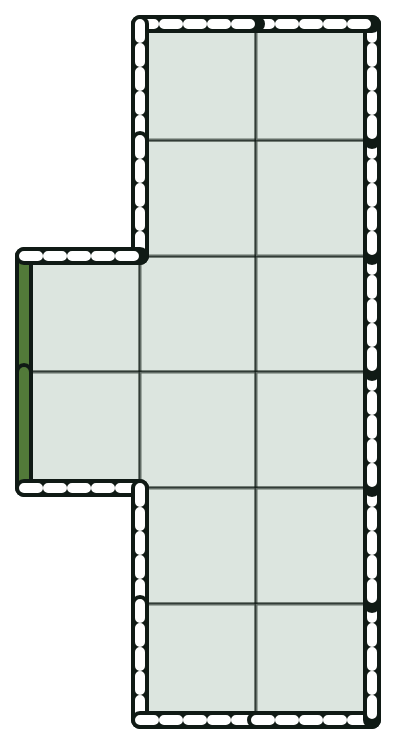
\includegraphics[height=5.2cm]{transizione-quadrati.png}\\[0.5em]
(a) Quadrati: $N=14$, $B=18$, $I=19$
\end{minipage}\hfill
\begin{minipage}[c]{0.45\textwidth}
\centering
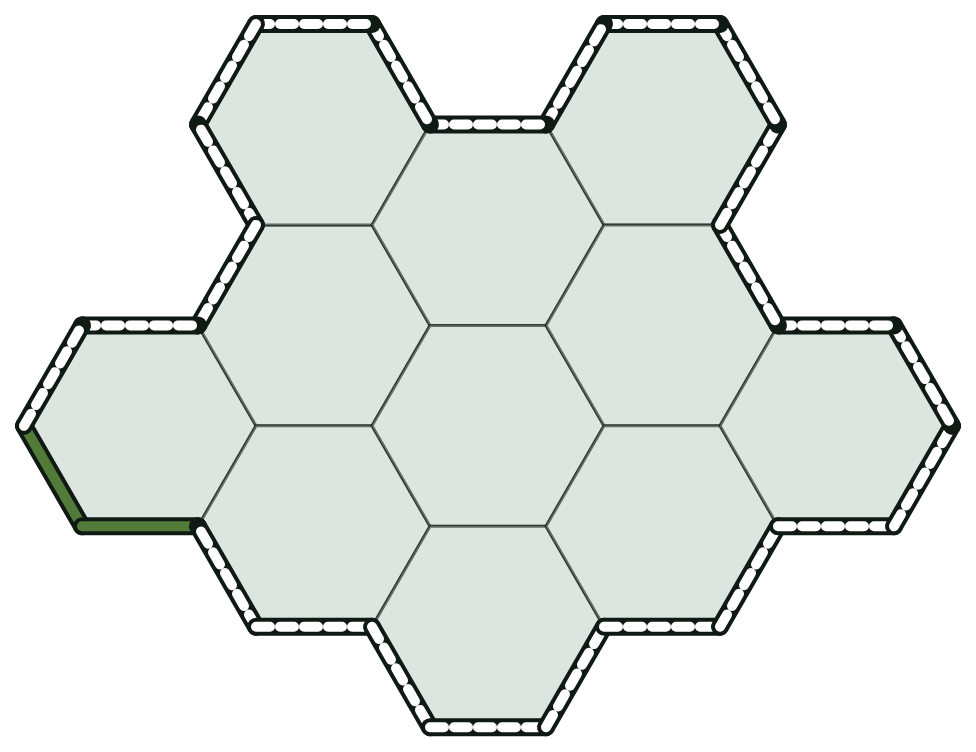
\includegraphics[height=3.7165cm]{transizione-esagoni.png}\\[0.5em]
(b) Esagoni: $N=11$, $B=26$, $I=20$
\end{minipage}
\caption{Realizzazione ottenuta e applicata nell'editor con $\varepsilon=30\%$, $\tau=50\%$ e modalità di forma disattivate. I due lati verdi restano singoli; le interfacce senza vincolo assorbono gli otto lati aggiuntivi. L'errore d'area è $\delta_A\simeq2{,}07\%$ e la deviazione del rapporto è $\delta_\rho\simeq27{,}13\%$. La figura mostra un candidato verificato del fronte trovato, senza certificazione di ottimalità globale.}
\label{fig:transizione}
\end{figure}

\subsection{Completezza rispetto allo spazio di interesse}

Possiamo ora formulare la domanda in modo distinto per ciascun livello. Per ogni forma $S$ che ammette almeno una coppia $(S,p)\in\mathcal R_{s'}^{\vartheta}(X)$, l'enumeratore astratto ha un percorso che la raggiunge. La corrispondenza deterministica scelta dall'editor soddisfa a sua volta i vincoli di bordo quando la capacità del perimetro è sufficiente, poiché le altre condizioni geometriche non dipendono da come si distribuiscono i lati senza vincolo.

Tuttavia, l'editor non restituisce tutte queste forme: può arrestarsi prima, non ammette le verifiche di forma inconcludenti quando il vincolo è attivo, elimina i risultati numericamente dominati e limita i rappresentanti geometrici. La preferenza continua cambia la priorità di scoperta; non rende esaustiva la procedura né elimina i limiti numerici. Inoltre, anche eliminando i limiti di risorse e il filtro Pareto, la sola corrispondenza deterministica non copre tutte le realizzazioni di bordo ammissibili.

Rimane quindi interessante confrontare una modalità che seleziona pochi rappresentanti con una modalità esaustiva, limitata a istanze abbastanza piccole, che enumeri tutte le distribuzioni e gli allineamenti di bordo ammessi. Occorrerà precisare quali differenze si vogliono identificare come equivalenze, prima di confrontare il numero delle realizzazioni raggiunte.

\subsection{Primo confronto con una sorgente non convessa}
\label{sec:esperimento-c}

Un primo esperimento usa una C di $13$ quadrati, con due bracci orizzontali di cinque celle e una colonna sinistra di collegamento. La sorgente ha $B=28$, $I=12$ e tutte le interfacce senza vincolo. La destinazione è esagonale, con $\varepsilon=30\%$, $\tau=50\%$, $p_\sigma=10$ e vincolo di forma disattivato. Si confrontano $\alpha=0$ e $\alpha=1$ con lo stesso budget di $6000$ avanzamenti dei generatori. Un avanzamento è un'unità di lavoro della procedura, non una durata uguale nei due casi.

La ricerca originaria esamina $48$ insiemi distinti e ammette $23$ candidati, mantenendo un rappresentante. La ricerca con preferenza geometrica ne esamina $60$ e ne ammette $33$, mantenendo $18$ rappresentanti. I risultati della figura~\ref{fig:campo-c} sono generati, verificati e visualizzati in Wang Studio. La regione blu è il riferimento continuo; la tassellazione verde è la destinazione, sovrapposta dopo l'allineamento dei centroidi.

\begin{figure}[htbp]
\centering
\begin{minipage}[t]{0.32\textwidth}
\centering
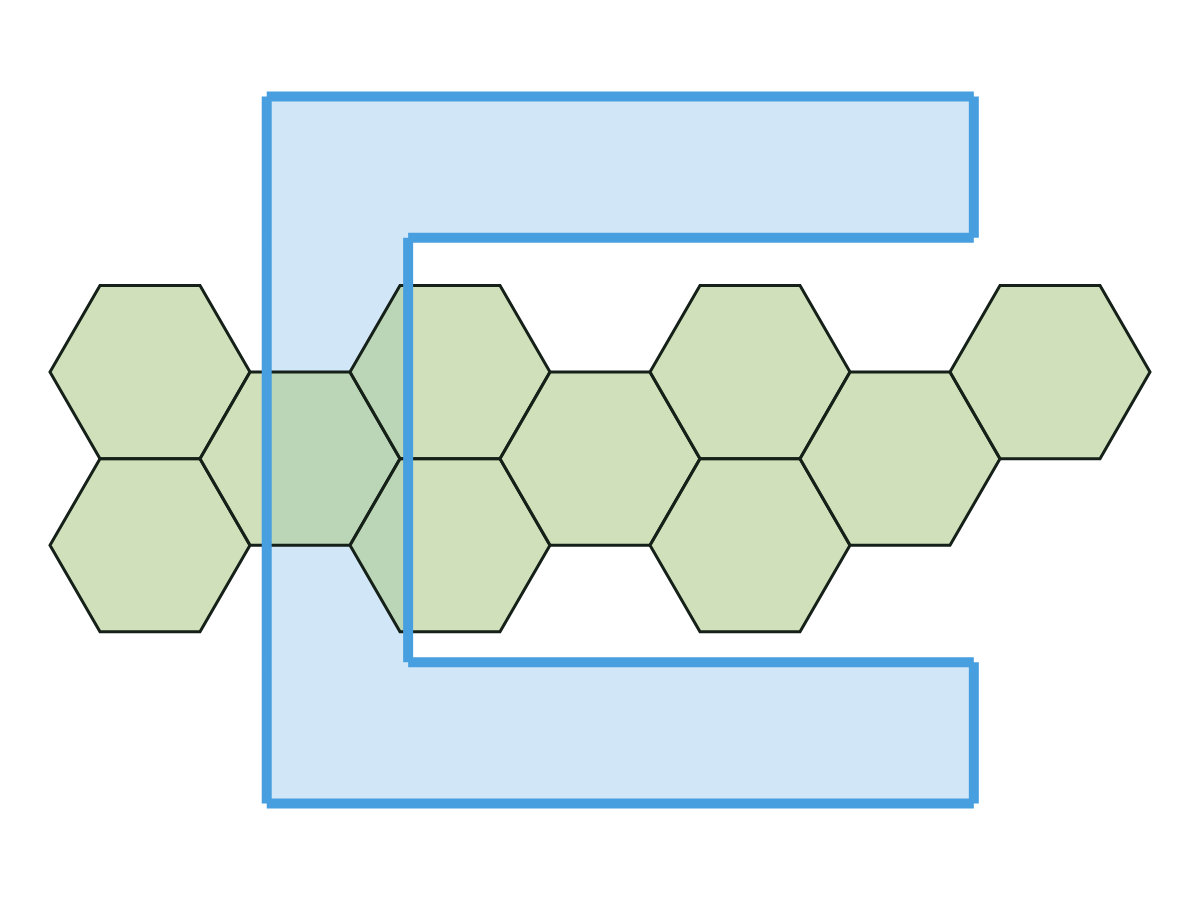
\includegraphics[width=\linewidth]{campo-c-non-guidata.png}\\[0.3em]
(a) Senza guida, $N=10$
\end{minipage}\hfill
\begin{minipage}[t]{0.32\textwidth}
\centering
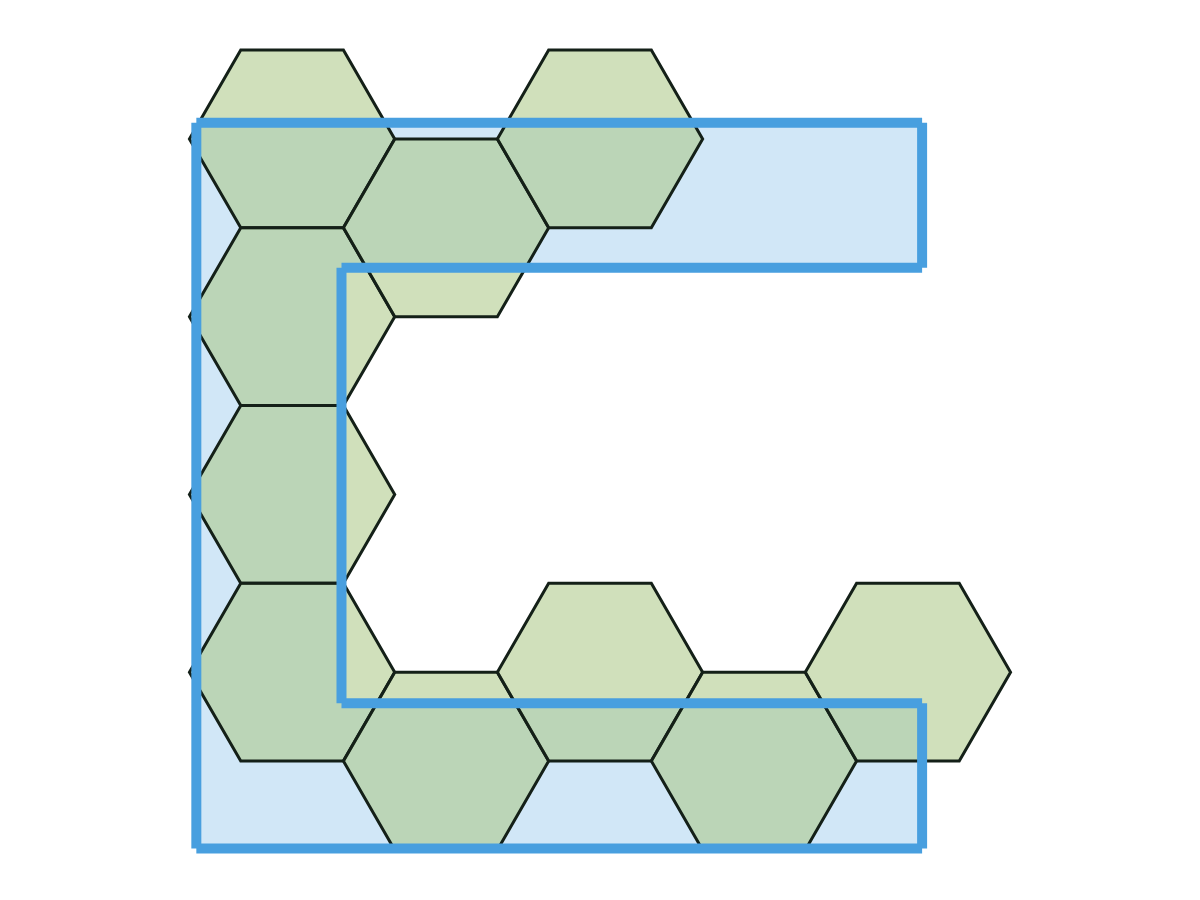
\includegraphics[width=\linewidth]{campo-c-guidata.png}\\[0.3em]
(b) Con guida, $N=10$
\end{minipage}\hfill
\begin{minipage}[t]{0.32\textwidth}
\centering
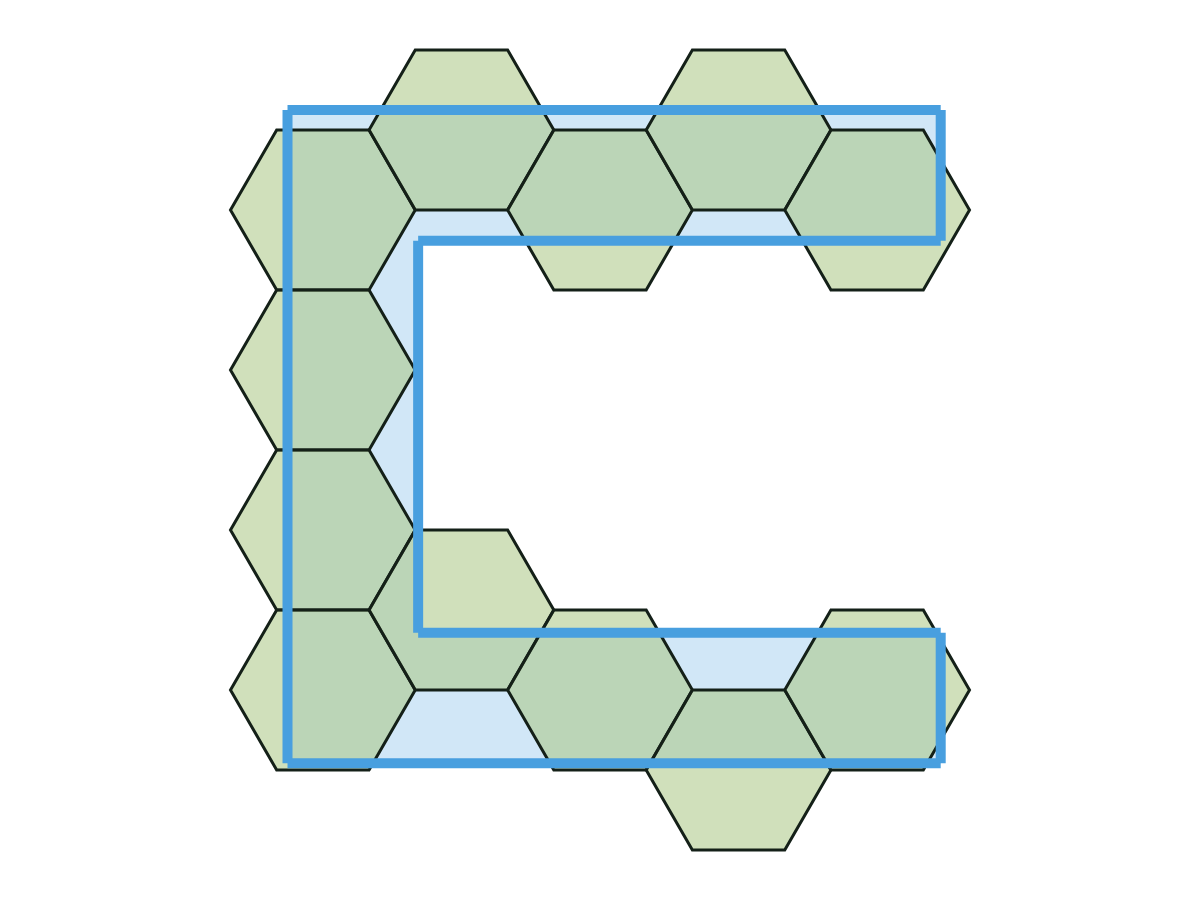
\includegraphics[width=\linewidth]{campo-c-forma.png}\\[0.3em]
(c) Con guida, $N=12$
\end{minipage}
\caption{Anteprime esportate da Wang Studio per la stessa sorgente a C e gli stessi vincoli d'area e $B/I$. La preferenza continua consente di trovare realizzazioni che seguono l'apertura e i bracci della sorgente. Il campo non obbliga a riprodurne esattamente il contorno. Ogni anteprima è adattata al proprio riquadro; le metriche usano lo stesso riferimento normalizzato. Il risultato (c) ha il minor punto medio dell'errore di forma fra i rappresentanti di questa ricerca; non è un ottimo globale certificato.}
\label{fig:campo-c}
\end{figure}

\begin{center}
\small
\begin{tabular}{lrrrr}
Realizzazione & $\delta_A$ & $\delta_\rho$ & $\widehat E_\sigma$ & $[L,U]$ \\
\hline
(a) Non guidata, 10 celle & $0{,}074\%$ & $2{,}04\%$ & $138{,}47\%$ & $[132{,}81;144{,}14]\%$ \\
(b) Guidata, 10 celle & $0{,}074\%$ & $41{,}67\%$ & $37{,}10\%$ & $[33{,}90;40{,}31]\%$ \\
(c) Guidata, 12 celle & $19{,}91\%$ & $41{,}67\%$ & $25{,}68\%$ & $[22{,}51;28{,}85]\%$
\end{tabular}
\end{center}

Gli intervalli riportati derivano da una rivalutazione comune con budget di $32768$ rettangoli, più ampio di quello usato durante la ricerca. Anche questo budget non raggiunge in tutti i casi la precisione richiesta: la tabella conserva l'incertezza residua, invece di presentare il punto medio come valore esatto.

Il confronto fra (a) e (b) mantiene la stessa area di destinazione, ma il miglioramento di forma si accompagna a una maggiore deviazione $B/I$, ancora entro il vincolo. Il risultato (c) impiega anche una parte maggiore della tolleranza d'area. Si osservano dunque compromessi distinti, non un miglioramento simultaneo di tutti gli obiettivi. In particolare il valore predefinito $p_E=30$ non è stato imposto: (b) supererebbe tale soglia, mentre per (c) l'intervallo più raffinato ne indica il rispetto. Questo non implica che il verificatore con budget ordinario riuscirebbe a concluderlo.

Le figure sono accompagnate dai progetti ricaricabili e dai dati di generazione della sessione Chromium. I conteggi si riferiscono a questa esecuzione: una precedente esecuzione in Node, con lo stesso budget nominale, ha prodotto conteggi leggermente diversi ma gli stessi tre valori riportati in tabella alla precisione mostrata. Il budget da solo non garantisce riproducibilità identica fra ambienti numerici diversi; va conservata anche la versione dell'ambiente di esecuzione. Il confronto suggerisce di proseguire con regioni a U, rientranze strette e forme asimmetriche, misurando separatamente qualità delle realizzazioni, costo della ricerca e precisione della verifica numerica.

\section{Misure di complessità ed espressività}

Definito lo spazio dei problemi e introdotte delle metodologie per muoversi al suo interno, si presenta la necessità di definire quantità che permettano di confrontare le proprietà delle istanze.

Si vorrebbero ricercare due funzioni
\[
H_C:\mathcal P\to\mathbb R,
\qquad H_E:\mathcal P\to\mathbb R,
\]
rappresentative rispettivamente della complessità e dell'espressività, dove $\mathcal P$ è lo spazio delle istanze definito in precedenza. La definizione di queste misure e delle loro relazioni costituisce un obiettivo della ricerca.

Tempo di esecuzione, nodi visitati e memoria saranno osservabili sperimentali da confrontare a solver, rappresentazione e ambiente fissati.

Le famiglie con complessità nota offriranno un riferimento per lo studio delle misure. Un primo esempio è il problema NP-completo di tassellare regioni semplicemente connesse con il tileset fissato di 23 Wang tiles di Yang e Zhang~\cite{yangzhang}.

Per espressività si vorrebbe comprendere quali configurazioni o computazioni una famiglia di tileset e regioni possa rappresentare e con quale costo di codifica.

Si ritiene interessante indagare se queste misure possano essere ricondotte a concetti di entropia. L'intuizione nasce dal fatto che un problema definisce uno spazio di configurazioni e impone vincoli che ne selezionano un sottoinsieme. Si vorrebbe studiare quanto la struttura di tale spazio rifletta l'espressività e la difficoltà di risoluzione.

Una prima richiesta per le misure sarà chiarire quali equivalenze debbano rispettare, come la rinomina dei colori e la traslazione dell'intera regione. Si vorrebbe poi studiare se le quantità proposte distinguano effettivamente famiglie con comportamenti noti e se permettano di interpretare l'effetto delle variazioni dei vincoli.

\section{Studio numerico e ruolo dell'editor}

Si ritiene interessante condurre uno studio numerico delle distribuzioni delle proprietà osservabili, delle relazioni fra vincoli e del comportamento durante le transizioni. Si vorrebbero individuare regolarità, discontinuità ed eventuali fenomeni di soglia.

Ogni esperimento fisserà geometria, dimensioni delle regioni, numero di colori, regola di costruzione del tileset e condizioni di bordo, insieme alle simmetrie identificate e alla distribuzione di campionamento.

Per ciascuna istanza si conserveranno dati del problema, parametri di generazione, versione del solver ed esito, distinguendo conteggi esatti e risultati parziali.

\subsection{Stato del prototipo}

Wang Studio permette di costruire regioni, palette e tileset atomici su griglie quadrate, triangolari ed esagonali; impostare bordi colorati o senza vincolo; salvare i progetti ed esportare immagini. Integra i solver di Tiling Foundry tramite le adiacenze delle griglie supportate, con ricerca della soluzione successiva e conteggio completo quando la ricerca termina.

La ricerca geometrica fra le tre famiglie è distinta dalla risoluzione del problema di tiling. La gestione di tessere generalizzate con verifica dell'unicità e posizionamento come pezzi indivisibili rimane da implementare.

La transizione descritta comprende il campo continuo, le due modalità di forma e l'anteprima sovrapposta della versione di lavoro dell'11 ottobre 2026; la copia pubblicata può precedere questa revisione.

L'editor è accessibile all'indirizzo
\begin{center}
\url{https://xtraid.github.io/wang-studio/}
\end{center}
e il sorgente è disponibile in
\begin{center}
\url{https://github.com/xtraid/wang-studio}.
\end{center}

\subsection{Prime domande e percorso di lavoro}

Fatte queste premesse, propongo di iniziare da famiglie piccole per le quali sia possibile verificare esaustivamente sia le soluzioni sia lo spazio delle realizzazioni geometriche. Questo permetterebbe di confrontare le scelte dell'editor con un riferimento completo, prima di estendere gli esperimenti.

Le prime domande che ritengo rilevanti sono:
\begin{enumerate}
\item Quali equivalenze fra istanze sono utili per eliminare differenze di sola rappresentazione senza perdere proprietà di interesse?
\item Quali variazioni dei vincoli modificano tesserabilità, numero delle soluzioni e costo della ricerca, e con quali dipendenze reciproche?
\item Quanto incidono la scelta della corrispondenza di bordo e la politica sul tileset nei confronti fra geometrie? Quando si può costruire una transizione che conservi anche proprietà delle soluzioni?
\item Quanto incidono larghezza della fascia, soglia di forma e precisione dell'integrale sulla qualità delle realizzazioni e sul costo della ricerca? Quali compromessi emergono rispetto ad area e rapporto di contatto?
\item Quali vincoli permettono di utilizzare tessere generalizzate preservandone l'integrità e l'unicità della decomposizione?
\item Quali osservabili distinguono famiglie note e quali possono contribuire a una definizione verificabile di complessità o espressività?
\end{enumerate}

Il risultato atteso da questa prima fase è una definizione sufficientemente precisa dello spazio e delle operazioni, accompagnata da un insieme riproducibile di istanze ed esperimenti. Si auspica che questo permetta di scegliere, insieme al supervisore, quali sottoinsiemi e quali proprietà approfondire.

\begin{thebibliography}{9}
\bibitem{berger}
Robert Berger.
\emph{The Undecidability of the Domino Problem}.
Memoirs of the American Mathematical Society, n.~66, 1966.
\href{https://doi.org/10.1090/MEMO/0066}{doi:10.1090/MEMO/0066}.

\bibitem{yangzhang}
Chao Yang e Zhujun Zhang.
\emph{NP-completeness of Tiling Finite Simply Connected Regions with a Fixed Set of Wang Tiles}.
arXiv:2405.01017, versione 2, 2024.
\url{https://arxiv.org/abs/2405.01017v2}.
\end{thebibliography}
\end{document}
